\documentclass[11pt]{article}
% \usepackage[margin=1in]{geometry}
\usepackage{enumerate}
\usepackage{forest}
\usepackage[margin=1in]{geometry}
\usepackage{mathtools}
\usepackage{amsmath}
\usepackage{amssymb}
\usepackage{gensymb}
\usepackage{hyperref}

%opening
\title{CSCI 491/591 P2}
\date{March 1, 2016}
\author{Group 4\\Chenglin Fan, Jici Huang,
Angelica Davis, Peng Zou}

\begin{document}

\maketitle
\noindent
In the deliverable, we selected an interesting data set
that we will investigate in the project.  The data set is GPS trajectories. We will explain where the data is
from,  what  the  data  means,  and  conjecture  what  we  might  find  in  this
project.
\section*{Data Set Choice}
The data set being explored is a compilation of GPS trajectories extracted from the files discussed in P1. \\
In P1, we went through all data sets provided by Map Construction Portal and we decided to investigate trajectory data of the tracks in Berlin, large. It is a suitable representative data set because the size of trajectory data is about midway between Chicago and Athens. The data set size is a suitably comparable characteristic since the data sets represent overlapping trajectories as well as noisy trajectories. Thus, a mid-sized data set may well represent the noise ratio (either due to noisy trajectories or sampling uniformity).
% Data set choice (8 points). You must select an interesting data set
% that you will investigate in this project. The data set can be real (GPS trajectories,
% Four-square check-ins, gene expressions, March madness brackets,
% baseball statistics, 3D objects, movie scripts, etc.), or it can be theoretical
% (flip graphs, the space of image patches, etc.). [Deliverable: one-to-two page write-up].

\section*{Details About the Data}
The original data set files were downloaded from the Map Construction Portal with the website url as \url{http://www.mapconstruction.org/data_downloads/}.  The downloaded data set includes the tracking data of Berlin city. The data set has 27,189 trips (a trip is a collection of GPS trajectories for one trip over some time period) in .txt format. Each trip has three column numbers, and each column corresponds to x-coordinate, y-coordinate and time stamp corresponding to the x,y-coordinate. The following Table \ref{table:questions} will provide a brief description of the tracking data of Berlin city.
% Explain where the data is
% from, what the data means,
% TODO: write something here.\\
% \begin{center}
%  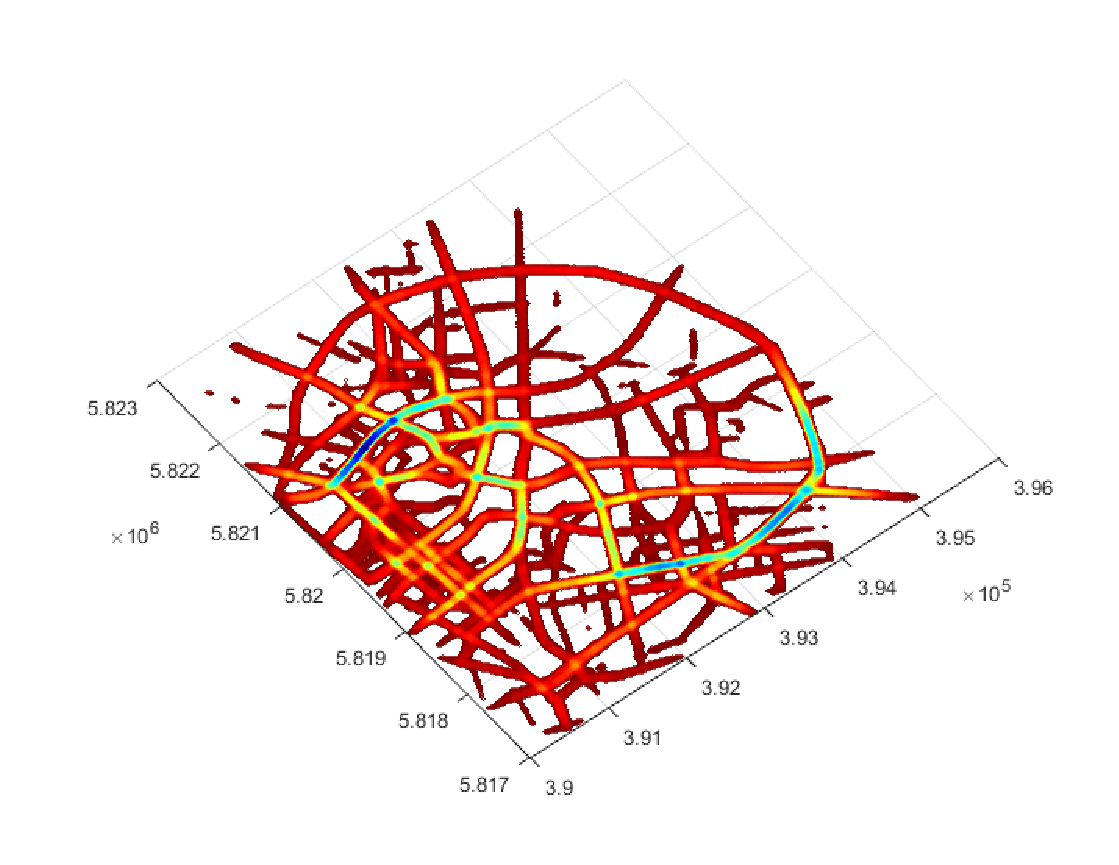
\includegraphics[scale=0.9]{p1.eps} 
% \end{center}
\begin{table}
\begin{center}
\begin{tabular}{ |l |c| r| }
\hline
  x-coordinate & y-coordinate & time stamp   \\ \hline
  393742.586772 & 5821049.184616 & 2585542.00   \\ \hline
  393747.949682 & 5821296.284551 & 2585604.00 \\  \hline
  393883.091662 & 5821448.203015 & 2585677.00  \\ \hline
  393759.343945 & 5821821.259046 & 2585738.00\\ \hline
  \vdots & \vdots & \vdots \\ \hline
\end{tabular}
\end{center}
\caption{Excerpt of track data of Berlin large in trip1}
\label{table:questions}
\end{table}

\begin{figure}[h!]
  \caption{A tracking map after processing the track Berlin large data set}
  \centering
 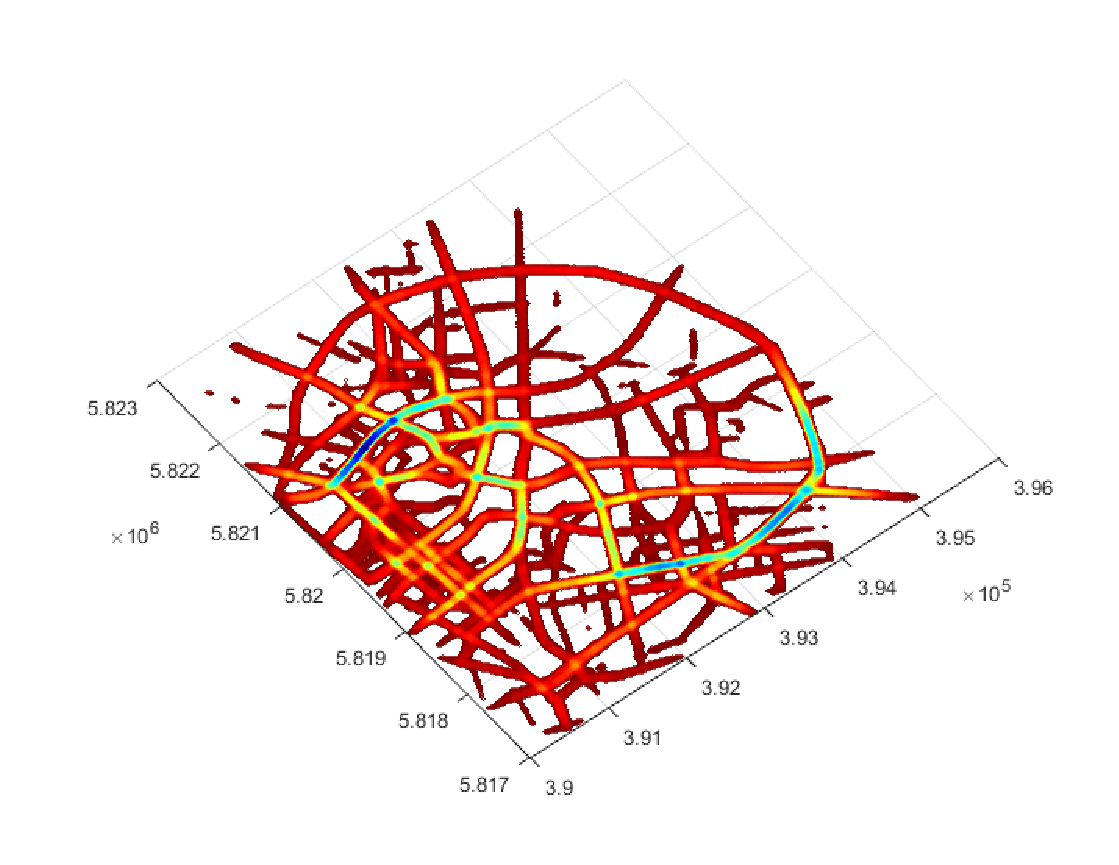
\includegraphics[scale=0.8]{p1.eps} 
\end{figure}

\pagebreak
\section*{Conjectures}

Explain where the data is
from, what the data means, and  {\em conjecture what you might find in this
project}.

\section*{Discussion}
In P2, we had discussion on the analysis of the data. We came up with two data files from the original trip files. \\
It is usually nice to conclude any write-up.\\

pts.txt: grid points after the city, 
manifold value: clr.txt
\section*{Conclusion}

\end{document}
